%------------------------------------------------------------------------
%
%  Labtainer Student Guide
%
%  Author: Michael Thompson
%
%  NOTICE: This document was developed for the Labtainer framework by the 
%  Naval Postgraduate School, Center for Cybersecurity and Cyber Operations 
%  under National Science Foundation Award No. 1438893. 
%  This work is in the public domain, and cannot be copyrighted.
%------------------------------------------------------------------------
\documentclass[12pt]{article}
\usepackage{geometry}
\geometry{a4paper, total={170mm,257mm},left=20mm, top=10mm,}
\usepackage[colorlinks=true,linkcolor=blue,urlcolor=black]{hyperref}
\usepackage{bookmark}
\usepackage{pdfpages}
\usepackage{graphicx}
\usepackage[autostyle, english = american]{csquotes}
\begin{document}
\begin{titlepage}
\centering
\vfill
\vspace*{4\baselineskip}
{\bfseries\Large
Labtainers Student Guide\par
}
\vspace*{4\baselineskip}
{\bfseries
Fully provisioned cybersecurity labs\par
}
\vspace*{2\baselineskip}
\today
\vfill
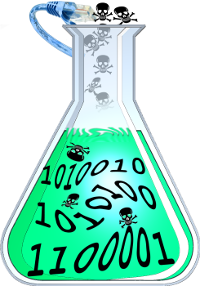
\includegraphics[width=2in]{labtainer5-sm.png}
  %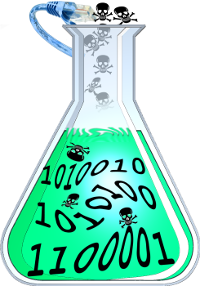
\includegraphics[width=\linewidth, scale=0.50,natwidth=200, natheight=286]{labtainer5-sm.png}
\vfill
\end{titlepage}

%----------------
\section {Introduction}
This manual is intended for use by students performing lab exercises with Labtainers.
Labtainers provide a fully provisioned execution environment for performing
cybersecurity laboratory exercises, including network topologies that include several different
interconnected computers.

Labtainers assume you have a Linux system, e.g., a virtual machine appliance described below.
If you are accessing a Labtainers VM via a web browser, you can skip to section \ref{performing}.

%----------------
\subsection{Obtaining and installing Labtainers}
Labtainers requires an x86-based computer.  It will not run on ARM-based processors such as 
Mac M1-based Powerbooks.

The easiest way to obtain Labtainers is to download one of the pre-configured virtual machines from
\url{https://nps.edu/web/c3o/virtual-machine-images}, and import it into either VirtualBox or VMWare.
Follow the brief instructions on that download page.  When you first boot the resulting VM,
Labtainers will take a moment to update itself.  You are then provided a terminal that includes
some hints, and can be used to run Labtainers.  

Note that the VM's Ubuntu Linux distribution is configured to NOT
automatically perform system updates.  It may prompt you to download and install updates.  That is typically
not necessary and may tie up your network bandwidth.  Yes, we are suggesting you not update your Linux
VM unless and until you have the time and the bandwidth.

You may now skip to section \ref{performing}.

\subsection{Alternatives to the Labtainers VM Appliance}
Skip this section and go to section \ref{selecting} if you are using a Labtainers VM appliance or accessing
Labtainers remotely via a browser.

\textbf{Please note} that Docker runs as a privileged service on your computer, and Labtainers containers run as privileged containers.
If you have sensitive data on your computer, you should understand the isolation provided by Dockers on your system.  An alternative
is to use one of our virtual machine appliances rather than running Docker directly on your computer.

\subsubsection{Installing Labtainers on an existing Linux system}
The Labtainer framework is distributed as a tarball from:
\url{https://nps.edu/web/c3o/labtainers}
Click the link named: ``Download the Labtainer framework'', and untar the resulting file into 
a permanent directory on your Linux system, e.g., into \verb ~/home.  For example, if you downloaded the file
from a browser on your Linux system:
\begin{verbatim}
   cd
   tar -xf ~/Downloads/labtainer.tar
\end{verbatim}
From the directory into which you untarred the
tarball start the installer script:
\begin{verbatim}
   cd labtainer
   ./install-labtainer.sh
\end{verbatim}

This script will install the latest version of Docker and packages required
by the Labtainer framework.  It will cause your Linux host to reboot when it
completes.

After the Linux host reboots, open a terminal to your Linux host and
change directory to wherever you untarred the tarball, e.g., your HOME directory.

\subsubsection{Docker Desktop on Mac and Windows}
This option assumes you have installed Docker Desktop and are familiar with its operation
and its security considerations.  Instead of using the window manager of your computer, this option lets you use a web browser
to interact with windows managed by the NOVNC program.  The window manager appears in your browser.

Download the script from \url{https://raw.githubusercontent.com/mfthomps/Labtainers/master/headless-lite/headless-labtainers.sh},
make it executable and run it.  On a Mac, this would be done from a terminal.  On Windows, use Powershell.
Open a browser and goto \url{http://localhost:6901/vnc.html?password=}
No password is needed, if prompted, simply click the submit button.

In addition to starting the Labtainers, the script will create a ~/headless-labtainers directory.  You should then run
{\tt headless-labtainers.sh} from that directory in the future to start Labtainers.  That directory will also contain persistent data, including
results stored in the {\tt labtainer\_xfer} subdirectory.  \textbf{Note:} Where lab messages and lab manuals indicate 
results are found in {\tt ~/labtainer\_xfer}, your results will be in {\tt ~/headless-labtainers/labtainer\_xfer}

Use {\tt ctrl-C} to quit Labtainers. 

\section{Selecting a Lab}
\label{selecting}
All labs are run from the same Labtainer workspace directory, which is typically at:
\begin{verbatim}
    cd $LABTAINER_DIR/scripts/labtainer-student
\end{verbatim}
\noindent The prepackaged virtual machines automatically start a terminal in this directory.

To see a list of available labs, run the {\tt labtainer} command with no arguments:
\begin{verbatim}
    labtainer 
\end{verbatim}
\noindent Use the {\tt -k} option to see a list of searchable keywords, and the {\tt -f <keyword>} option to view a summary
of labs having that keyword.

Lab exercises are also organized into \textit{Labpacks} that are a collection multiple related labs that you may
wish to perform in sequence (e.g., based on direction from your instructor.)  Use the
\begin{verbatim}
    labpack
\end{verbatim}
\noindent to view a list of Lab Packs, and provide the name of a Labpack as an argument to see a list of the labs
within a Labpack.  That command output also includes an indication ({\tt [Y] or [N]}) of whether you've generated any results from 
each lab.  Your instructor may provide you with custom Labpacks in the form of a URL.  You may add those to your system by
using the 
\begin{verbatim}
    labpack -a <url>
\end{verbatim}

Your instructor may direct you to add new or custom lab exercises to your installation by providing you with a URL of an \textit{IModule}.
To get access to those labs, use:
\begin{verbatim}
    imodule <url>
\end{verbatim}

\section{Performing a Lab}
\label{performing}

To run a specific lab, include the name of the lab in the {\tt labtainer} command:
\begin{verbatim}
    labtainer <labname>
\end{verbatim}
\noindent where \textit{labname} is the name of the lab to run.  

Most labs direct you to a PDF version of a lab manual, which can usually 
be viewed by right clicking on the displayed path, or you can open the file in a browser.
Please note that some of the initial lab instructions repeat the steps you've already taken, and you need
not perform those again. 

A list of labtainer commands can be found in Appendix A of this document. 

Once you start the lab, you will typically see one or more virtual terminals connected to computers within
the lab.  While running the lab, if you require more virtual terminals, use:
\begin{verbatim}
    moreterm.py <labname> <container>
\end{verbatim}
\noindent where \textit{container} is the host name of the component on which to attach a terminal.  
It can be omitted for labs having a single component.

The virtual terminals for most labs present bash shells via which you can interact
with the attached computer, (which is actually a Docker container designed to appear
like a separate computer).  A single computer
may have multiple virtual terminals attached to it.  Each computer is independent, and 
may use networks to interact with other Labtainer computers within the lab.  

Many labs automatically gather results of your work, which you will provide to your instructor.
Note that, unless otherwise directed, exploration and experimentation you perform either before
or after performing the expected activity will not diminish or dilute your results.  And you typically
do not have to take actions to collect or record your results.  This occurs automatically as noted in the next section.  

%----------------
\subsection{Interrupting and Completing  Labs}
When you want to stop working for a while or are finished and ready to turn it in to your instructor, type:
\begin{verbatim}
    stoplab
\end{verbatim}

\noindent from the Linux system from which you issued the {\tt labtainer} command. All changes to the files, etc. will be preserved and you will be able to resume the lab just the way you started it. You can resume your work, as needed.

The {\tt stoplab }command always displays the directory containing a zip file that should be provided to your instructor. It shows the current results of your work. 

The easiest way to forward the complete zip file to the instructor is to start a browser, e.g., Firefox, on the VM from which you
are running Labtainers.  Then use the browser to either email the zip file, or upload it into an LMS system, e.g., Sakai.
Alternately, you can configure the VM to use a shared folder, and use that to copy the zip file to the host computer.

%----------------
\subsection{Redoing a Lab}
Sometimes you might want to redo the lab from the beginning.  In this case, type:
\begin{verbatim}
    labtainer -r  <labname>
\end{verbatim}
This will delete any previous containers associated with this lab and start it fresh.  \textbf{Warning}: this will cause all previous data from the named lab to be lost.

%----------------
\subsection{Checking your work}
Some labs include criteria by which to automatically assess your progress.
Where enabled and supported, this feature can be utilized by issuing the {\tt checkwork} command from Linux system.
That command can be run while the lab is still running.

%----------------
\subsection{Getting Help and Things to Avoid}
To get help, type:
\begin{verbatim}
    labtainer -h
\end{verbatim}
\noindent from the Linux system from which you issued the {\tt labtainer} command. A list of useful labtainer commands will be displayed.

Do not run multiple labs simultaneously.  Consistent results cannot be guaranteed when more than one lab runs at the same time.

%----------------
\subsection{Networking}
In addition to network properties defined for the lab,
each component \texttt{/etc/host} file includes a ``my\_host entry'' that names
the host Linux.  Most containers will include a default gateway that
leads to the Linux host.  This allows students to scp files to/from the container and host.
It also allows the student to reach external networks, e.g., to fetch additional packages in
support of student exploration.

In some instances, the lab requires one or more components to a have different default route.
Typically, these components will include a \textit{togglegw.sh} script that the student
can use to toggle the default gateway between one that leads to the host, and one defined for the lab.
This allows students to add packages on components having lab-specific default gateways.
Use of the \textit{togglegw.sh} script is not necessary to reach the Linux host, (e.g., to scp files).

%----------------
\subsection{Installing and Using Labtainers Behind a Web Proxy}
If you are not behind a web proxy, ignore this section (most school environments
are not behind proxies). 
If you are behind a web proxy, Labtainer installation
requires that you have configured your Linux package management configuration to reflect
the proxy, e.g., the /etc/atp/apt.conf or /etc/dnf.conf files.  

Additionally, you will need to configure your Docker service as described at:
\url{https://docs.docker.com/engine/admin/systemd/#httphttps-proxy}
And set the HTTP\_PROXY environment variable to your proxy, e.g., 
\begin{verbatim}
HTTP_PROXY=http://myproxy:3128
\end{verbatim}
If you wish to use apt-get from within a container to add new software to a container, you
must first modify the container's /etc/apt/apt.conf file to reflect your proxy.

%----------------
\subsection{Limitations}
The Labtainer ``computers'' are individual Docker containers that are interconnected via virtual
networks.  These containers each share the Linux kernel of your host.  Thus, a change
to the kernel configuration on one computer, (e.g., enabling ASLR), will be visible on
other containers, as well as your host.

It is suggested that the student's Linux host be a virtual machine that is
not used for purposes requiring trust.  Software programs contained in cybersecurity lab
exercises are not, in general, trusted.  And while Docker containers provide namespace
isolation between the containers and the Linux host, the containers run as privileged.
Labtainers run as Docker containers and use the Docker group 
which is root-equivalent.  In other words, even though you start a Docker container
as a non-privileged user, software in the resulting container can modify the Linux host,
e.g., the VM.

The computers each include a ``local'' directory beneath the HOME directory.  This is used
by the Labtainer framework and includes results that get packaged up for forwarding to the
instructor.  Do not modify any files beneath the .local directory.  Otherwise, you can treat
those containers as Linux systems, and explore them.

Pasting multiple commands into a labtainer terminal may result in the not all of the
commands being executed.

\appendix 
\pagenumbering{Alph}
\setcounter{page}{3}
\section* {Appendix A: Labtainer Command Summary}
\label{sec:appendixA}
The following labtainer commands are available from the \texttt{labtainer/labtainer-student}
directory.  Most of these commands include a {\tt -h} option for help:
\begin{itemize}
\item \texttt{labtainer <lab> --}
Start the named lab.  If no name is given, a list of available labs will be displayed.
\item \texttt{stoplab  --} Stop the currently running lab.
\item \texttt{moreterm.py <lab> <container> --} create a new virtual terminal for the container.
\item \texttt{labtainer <lab> -r --}
Delete any previous containers associated with this lab and start it fresh.  \textbf{Warning}: this will lose any
previous data from the named lab.
\item \texttt{checkwork} -- Performs automated assessment for selected labs and provides you with information about your progress.
\item \texttt{quiz} -- Provides a quiz for selected labs to help prepare you to perform the lab.
\item \texttt{check\_nets.py} -- Runs diagnostics to potentially resolve Docker related problems.

\end{itemize}

Most labs display lab instructions in one of the windows that appears after the lab starts.  If those instructions
stop displaying, e.g., because ``q'' is pressed in that window, then type the following in a virtual terminal (e.g.,
in a new terminal created using the moreterm.py script:
\begin{verbatim}
    less instructions.txt
\end{verbatim}


\end{document}
